\section{Desenvolvimento arquitetural de software}

Ao dar sequência à proposta da equipe em utilizar a arquitetura de microsserviços, utilizou-se o Docker para criar containers em cada serviço específico com dependências necessárias para a utilização do mesmo. Em cada serviço existe um Dockerfile que contém a descrição das tecnologias, volumes e portas previamente definidas. Existe ainda um arquivo chamado Docker-compose que irá gerenciar todos os containers e irá facilitar o controle e monitoramento de cada serviço.

\subsection{Serviços desenvolvidos}

Para que o sistema funcione com êxito todos os serviços devem estar devidamente configurados em containers de acordo com a funcionalidade e responsabilidade de cada um.

\begin{enumerate}
	\item \textbf{Greenhouse}: Esse é o principal serviço, pois ele trabalha no gerenciamento dos containers, é o responsável por criar uma rede de conexão entre todos os serviços, e por isso na sua raiz da aplicação encontra-se o arquivo docker-compose.yml em que nele há um algoritmo que instancia todos os serviços do projeto.
	\item \textbf{WebService}: Nesse serviço encontra-se a API do projeto, portanto é um serviço único e diferenciado que irá tratar de responsabilizar de receber os dados por meio de simuladores ou dados reais por meio do servidor rabbitmq instalado na Rasberry pi. Ao receber esses dados, eles serão tratados e realização o parser para o formato JSON para que seja possível enviar respostas em uma linguagem que possa ser escutada pelo webApp, o frontend da aplicação. Utilizou-se o framework Python e Flask, juntamente com algumas dependência cruciais para o desenvolvimento da aplicação.
	\item \textbf{WebApp}: Esse serviço foi desenvolvido para o frontend da aplicação, dessa forma, foi instalado o node.js e npm que são dependências do ReactJS, o framework Javascript. Portanto, este escuta as requisições do servidor da API para o recebimento do JSON e o tratamento dos dados para componentes que sejam visíveis na interface da aplicação.
	\item \textbf{Postgres}: Para o Banco de Dados do projeto, utilizou-se o Postgres, sendo assim, foi necessário um serviço que armazene todos os dados do projeto. Com o auxílio da dependência python SQLAlchemy utilizada em cada módulos de microsserviço, foi possível facilitar a criação da base de dados e a vinculação das models para a criação das tabelas e facilidade em realizar consultas de qualquer microsserviço por meio de simples chamadas de métodos disponíveis no SQLAlchemy.
	\item \textbf{Simulators}: Para os testes da aplicação no início do projeto foi possível mocar os dados utilizando o serviço simulators, este gera dados randomizados e gera instâncias para os microsserviços responsáveis armazenar os dados no banco de dados, garantindo que toda a aplicação aconteça normalmente sem a necessidade previamente da RaspBerry pi.
	\item \textbf{Rabbit}: Uma ótima maneira de trabalhar com microsserviços é utilizando o rabbitmq que utiliza o protocolo AMQP para o incremento de filas dos dados recebidos do microsserviços. Sendo assim, este serviço é responsável por gerenciar todas as filas e se conectar com todos os microsserviços, por isso é essencial que ele esteja ativo juntamente com o serviço de banco de dados antes que qualquer outro microsserviço se inicie.
	\item \textbf{TemperatureServer}: Esse foi o primeiro microsserviço de integração desenvolvido, ele é responsável pelo recebimento da temperatura ambiente e pela conexão com o rabbit, esse relacionamento com o rabbit é para o incremento dos dados em uma fila.
	\item \textbf{HumidityServer}: Esse microsserviço, da mesma forma que o anterior é responsável pelo recebimento da umidade relativa do ar interna à estufa. Ao receber os dados é realizado a inserção dos dados no banco de dados paralela à conexão do rabbit.
	\item \textbf{IluminationServer}: Para o monitoramento da luminosidade, foi desenvolvido o microsserviço de iluminação, este deve receber os dados recebidos pelos sensores e tratar em formato booleano (verdadeiro ou falso) para ilustrar a ausência ou não de luz dentro da estufa. 
	\item \textbf{PhServer}: O monitoramento do Ph também se torna necessário na aplicação, seguindo a lógica dos outros microsserviços de integração, teremos um serviço chamado phServer que irá receber da RaspBerry pi os dados em tempo reali e realizar o tratamento para o banco de dados.
	\item \textbf{WaterTemperatureServer}:  Esse serviço é bem similar ao serviço de temperatura ambiente, pois o recebimento e tratamento dos dados são realizados praticamente da mesma forma, sendo assim o serviço de temperatura da água irá conectar com o rabbit, realizar a inserção dos dados no banco.
	\item \textbf{WaterLevelServer}: Esse serviço é responsável pelo troca de água automática da estufa. A integração necessita desse serviço para a coleta dos níveis de água e realizar o monitoramento para que, quando estiver em um nível de pH fora da faixa ideal, uma mensagem de notificação é enviada ao usuário e este tem a escolha de despejar a solução líquida contida no repositório líquido ou deixar conforme estar.
	\item \textbf{DrawerStatusServer}: Para a integração de abertura/fechamento da gaveta é necessário esse serviço, ele recebe e envia sinais por meio do rabbit para a Raspberry pi. Para o recebimento de sinais, há um monitoramento do estado da gaveta e para o envio de sinais o algoritmo confere se a porta está fechada, caso esteja, a gaveta não abre, se a porta estiver aberta, a gaveta abre e fecha normalmente.
	\item \textbf{Nginx}: Para trabalhar na configuração e carregamento de imagens foi necessário a utilização do Nginx e este cuida da configuração de pastas e portas das imagens recebidas pela integração da Raspberry pi e uma câmera que tira fotos em sequência e envia para o rabbitmq online na Amazon.
\end{enumerate}

\section{Deployment}

\subsection{Aplicação}

\begin{enumerate}
	\item \textbf{Login}. \\ O usuário deve estar autenticado para conseguir acessar nossa aplicação, sendo assim, após realizado o cadastro do usuário, previamente configurado no sistema, é possível fazer o login da aplicação.
	
	\item \textbf{Dashboard}. \\ Para a página inicial, iniciamos com um Dashboard que realiza monitoramento em tempo real de todos os sensores da estufa.
	
	\item \textbf{Relatórios}. \\ Para cada microsserviço de integração são gerados relatório para serem observados nos períodos de dia, mês e ano com suas respectivas médias.
	
	\item \textbf{Gráficos}. \\ Os gráficos são gerados para fins de tornar ao usuário uma melhor visualização dos dados pertinentes no relatório, sendo assim, os gráficos ilustram a alteração dos valores de acordo com o período escolhido no sistema.

	\item \textbf{Notificações}. \\ Sempre que os dados recebidos estiverem fora da faixa ideal definida para cada sensor, é enviado um alerta ao usuário para que ele possa corrigir..
	
\end{enumerate}

\subsection{Aplicação Web}

	\begin{figure}[H]
		\centering
		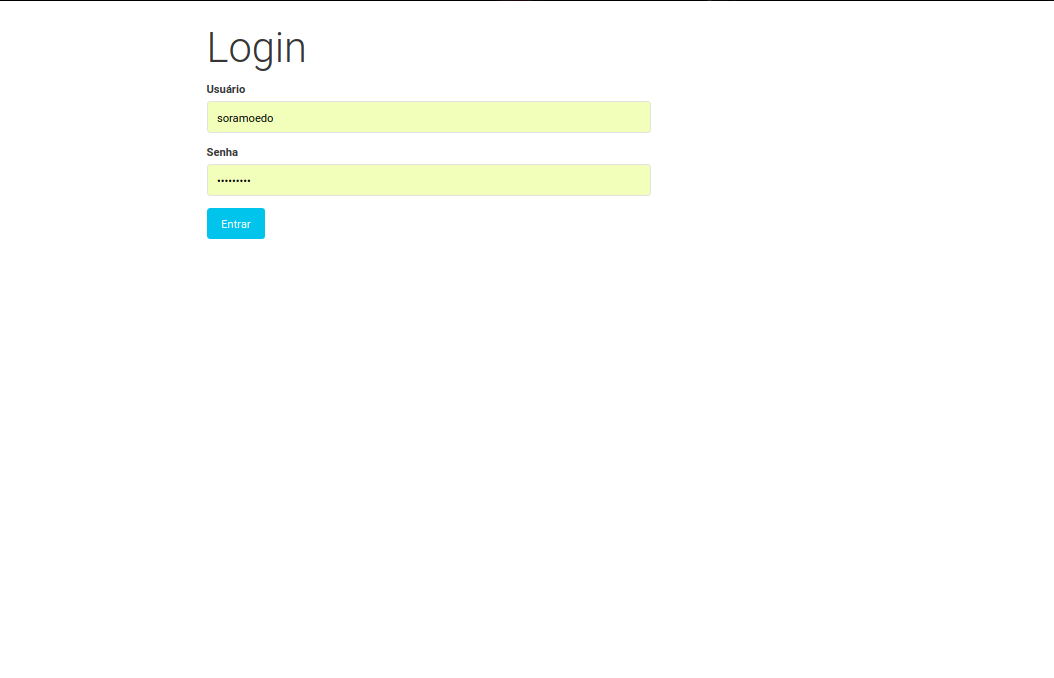
\includegraphics[width=10cm]{figuras/login.png}
		\caption{Tela de login.}
		\label{loginwebbapp}
	\end{figure}
	
	\begin{figure}[H]
		\centering
		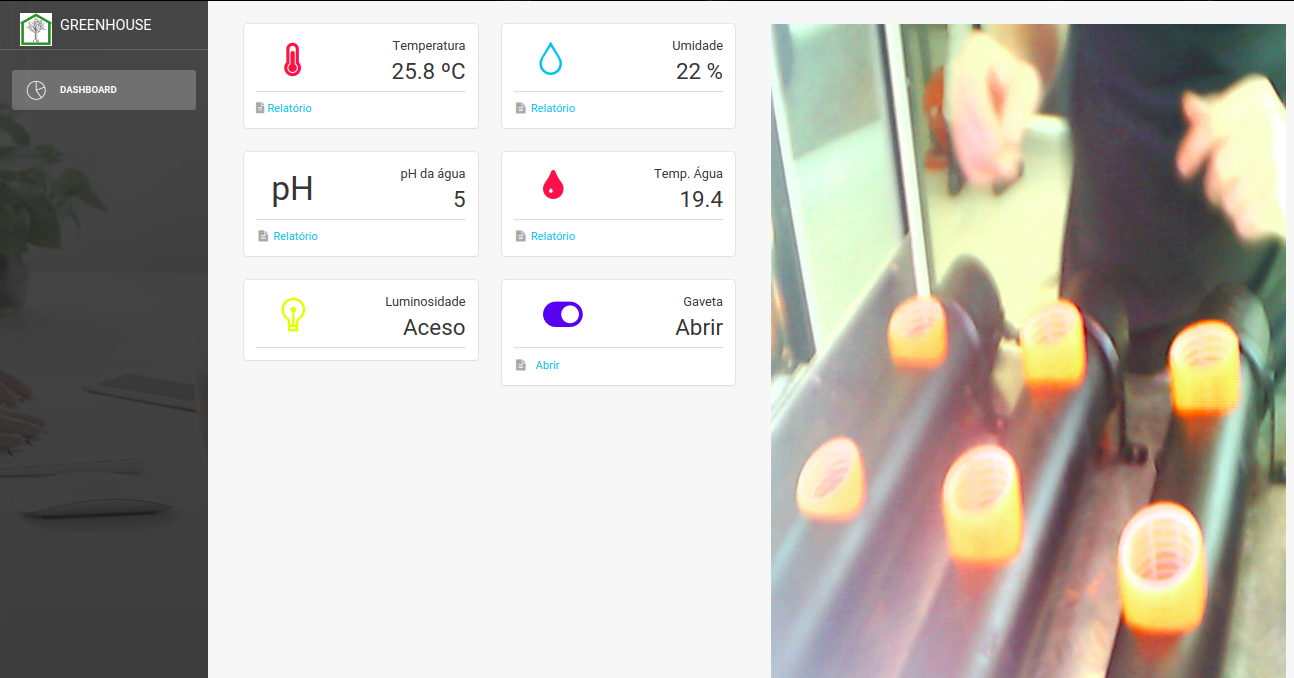
\includegraphics[width=10cm]{figuras/webapp.png}
		\caption{Tela inicial WebApp.}
		\label{webapp}
	\end{figure}
	
	\begin{figure}[H]
		\centering
		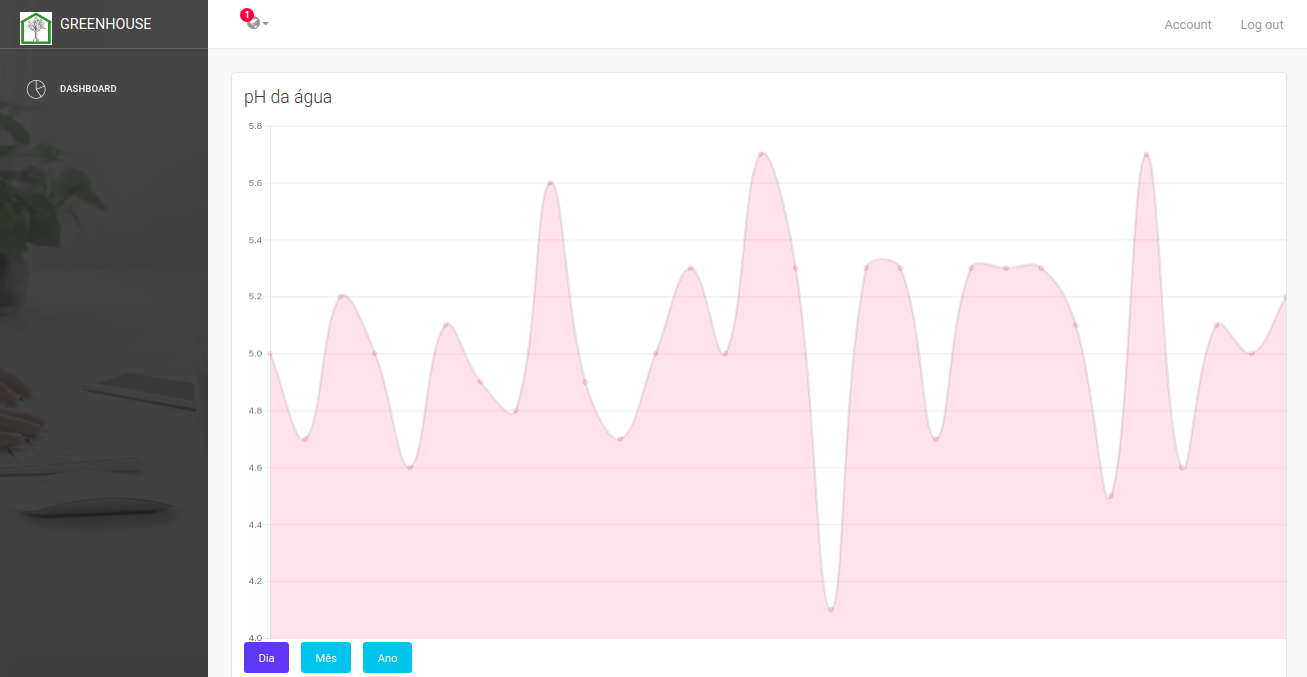
\includegraphics[width=10cm]{figuras/grafWeb.png}
		\caption{Gráfico no WebApp.}
		\label{grafweb}
	\end{figure}
	
\subsection{Aplicação Mobile}
	
	\begin{figure}[H]
		\centering
		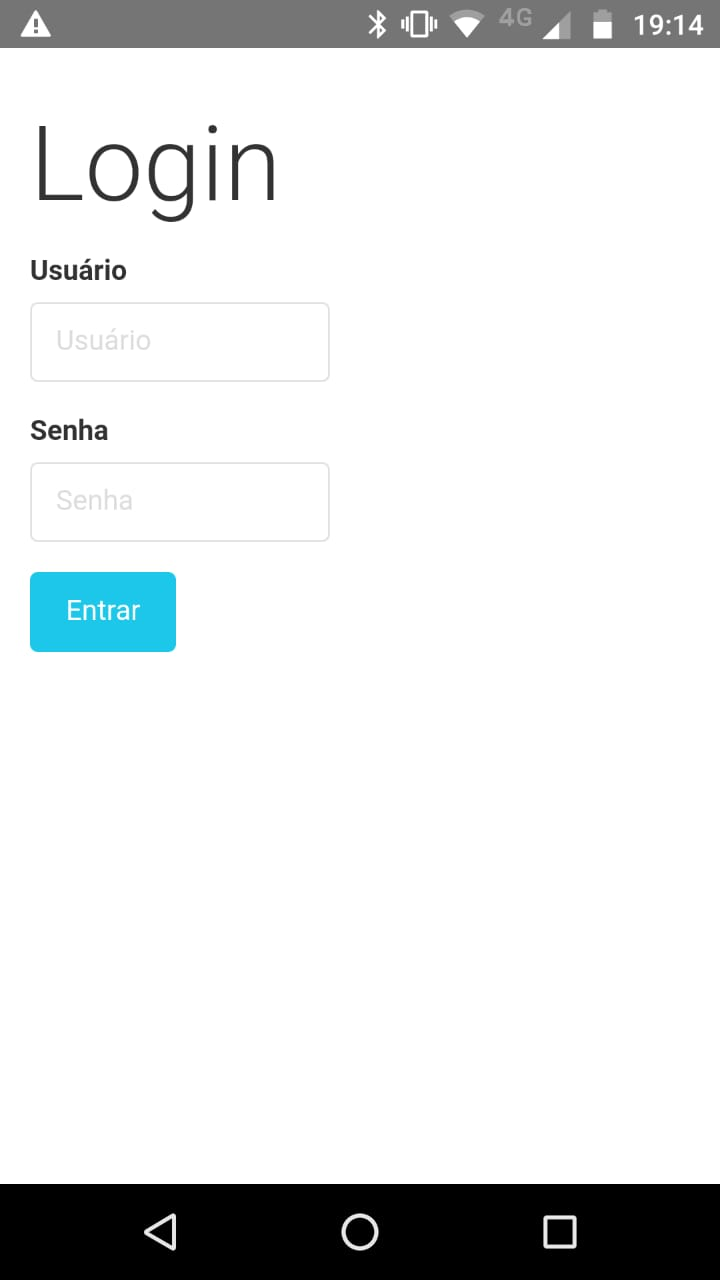
\includegraphics[width=5cm]{figuras/loginMob.jpeg}
		\caption{Login Mobile.}
		\label{loginMob}
	\end{figure}
	
	
	\begin{figure}[H]
		\centering
		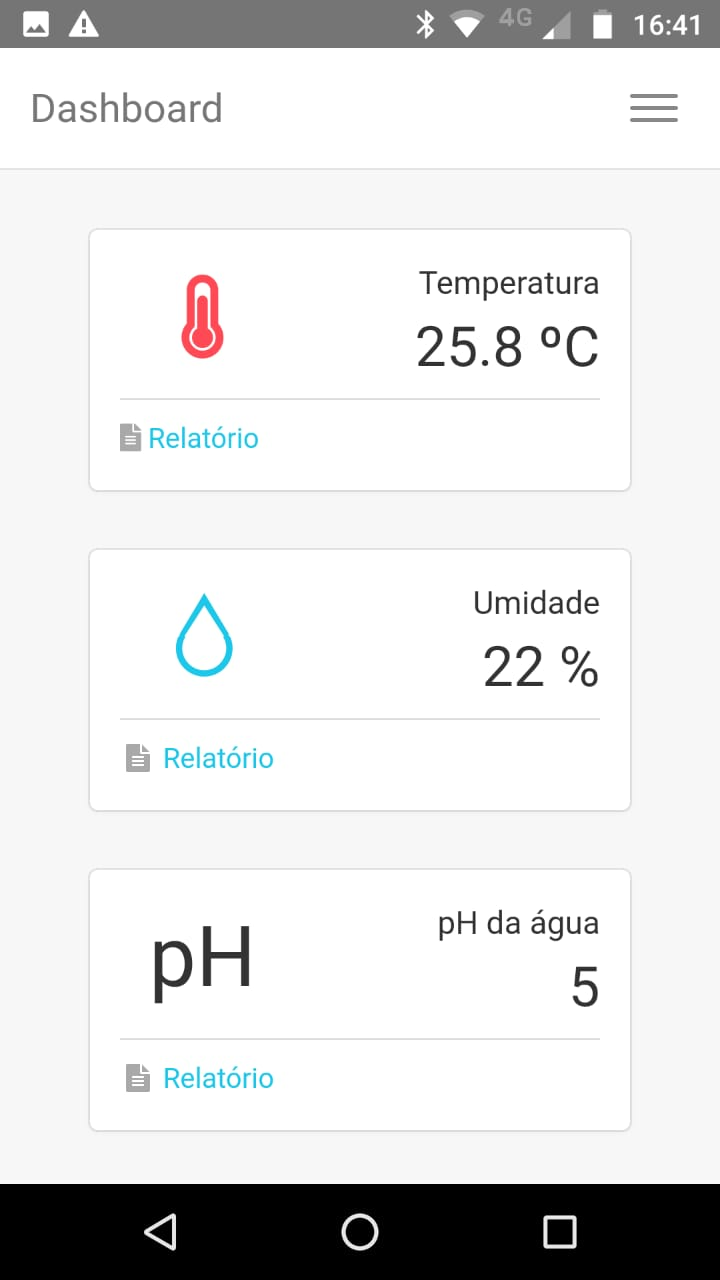
\includegraphics[width=5cm]{figuras/sensorMob.jpeg}
		\caption{Tela inicial Mobile.}
		\label{sensorMob}
	\end{figure}

	\begin{figure}[H]
		\centering
		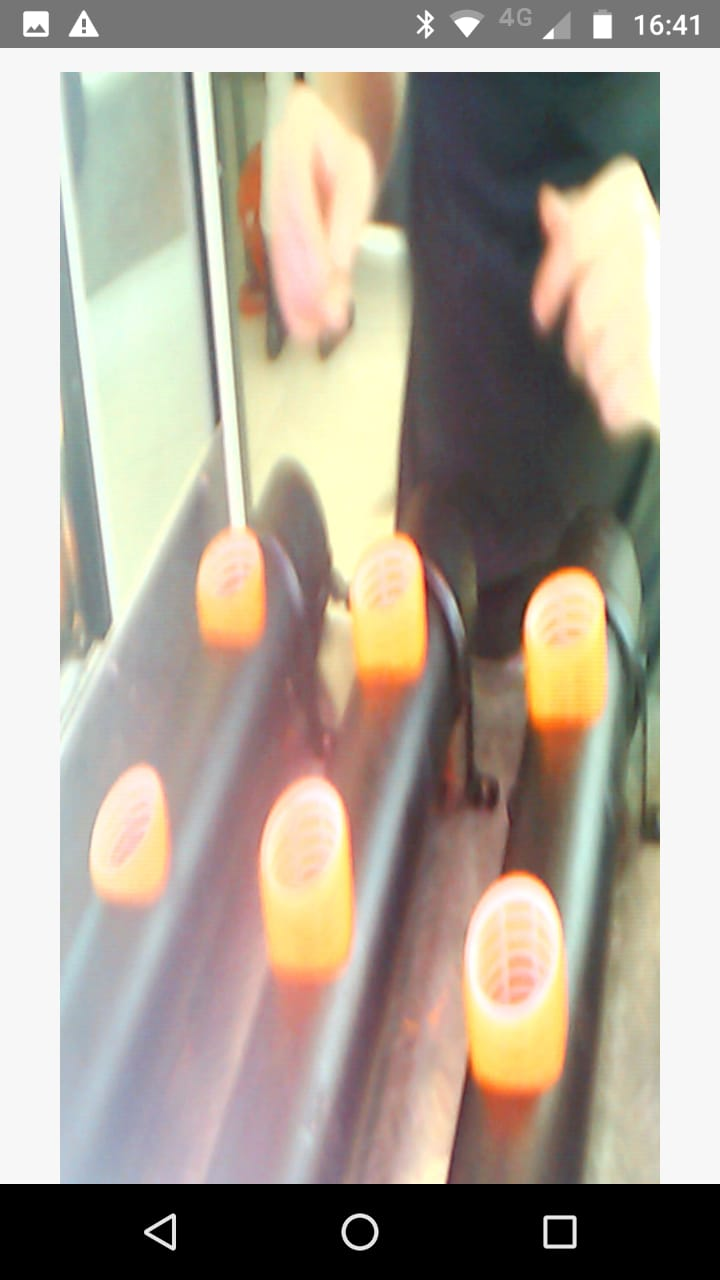
\includegraphics[width=5cm]{figuras/imagMob.jpeg}
		\caption{Imagem Mobile.}
		\label{imagMob}
	\end{figure}
	
	\begin{figure}[H]
		\centering
		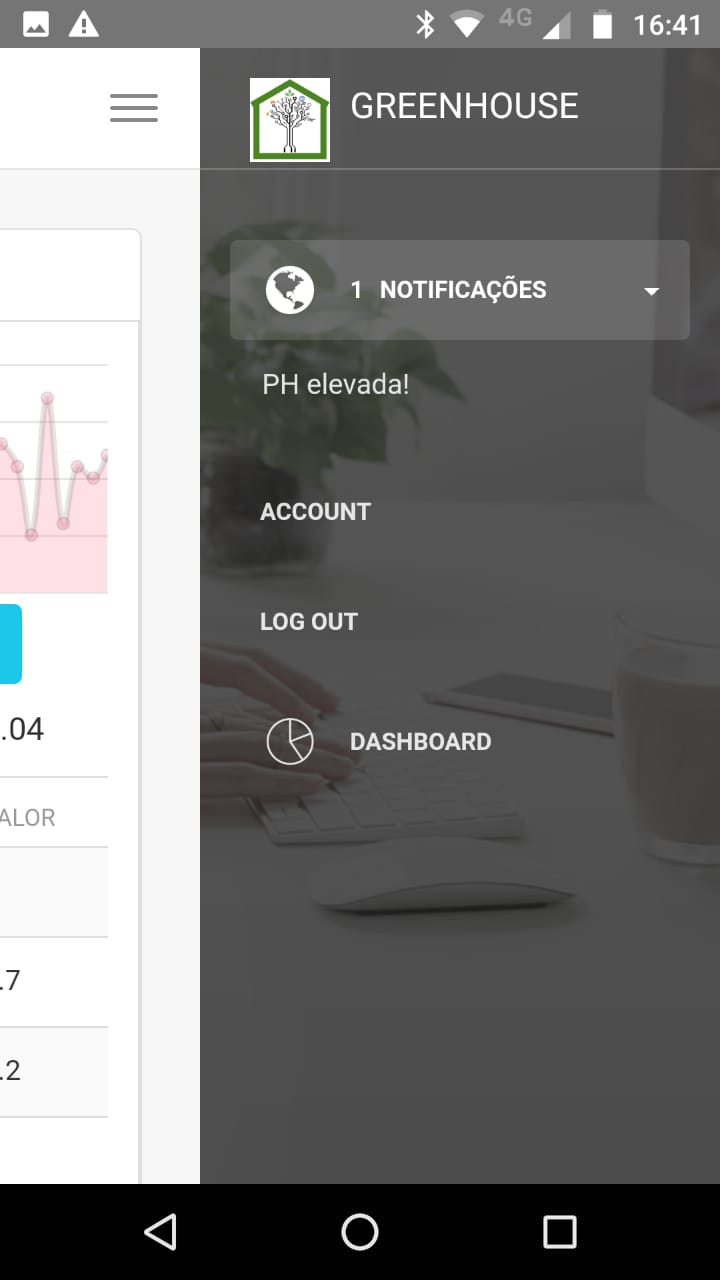
\includegraphics[width=5cm]{figuras/dashMob.jpeg}
		\caption{Dashboard Mobile.}
		\label{dashMob}
	\end{figure}
	
	
	\begin{figure}[H]
		\centering
		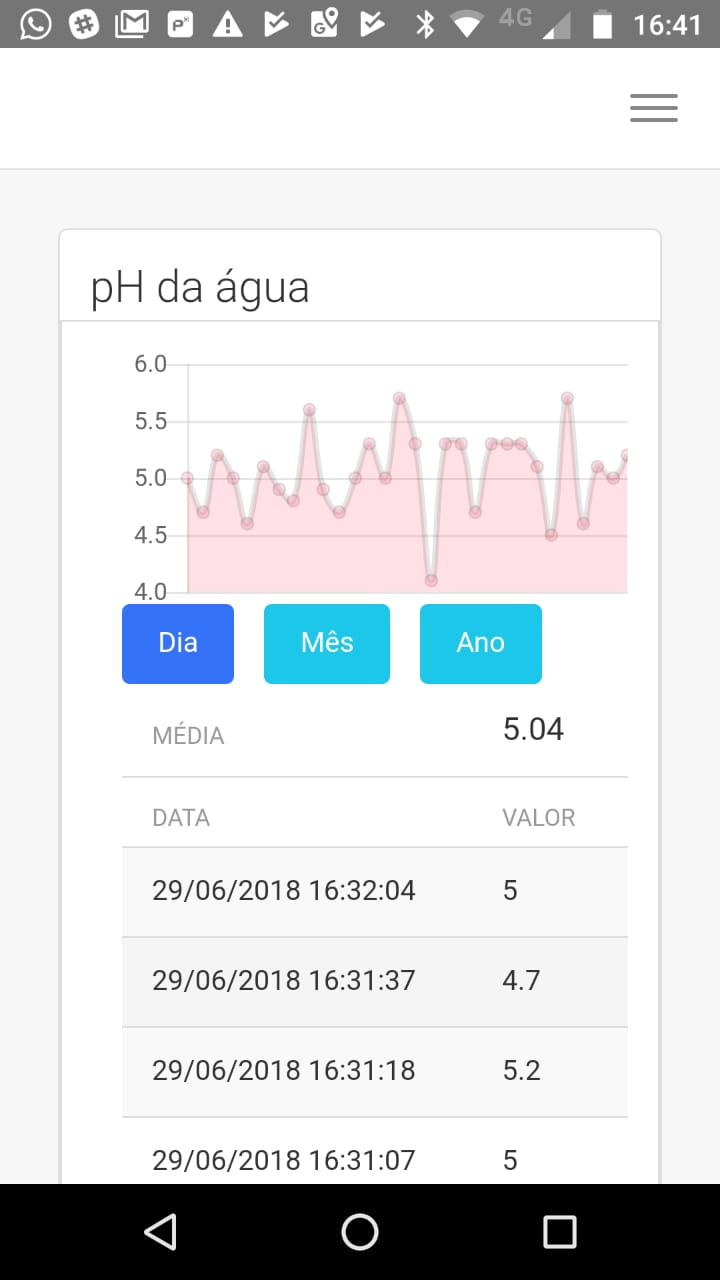
\includegraphics[width=5cm]{figuras/grafMob.jpeg}
		\caption{Gráfico no Mobile.}
		\label{grafmob}
	\end{figure}
